\section{Background: autoregressive vs block-diffusion decoding}
\label{sec:laws}

\subsection{How the two architectures decode}

\paragraph{Autoregressive (AR).}
The model generates output one token at a time. Each token requires a
forward pass over the full model and the growing KV cache; the model
can't begin token $t_{i+1}$ until it has finished $t_i$. The cost is
strictly sequential, one forward pass per token, no parallelism
within the sequence.

\paragraph{Block-diffusion (DG).}
The model generates an entire canvas of $C$ tokens in parallel
through $K$ iterative denoising passes. On each pass, the model
refines all $C$ token positions simultaneously: it starts from noise,
predicts cleaner tokens at every position, and repeats. After $K$
passes the canvas is fully decoded and the model steps to the next
canvas. Within a canvas, tokens are free, they are denoised in
parallel, so adding more tokens up to $C$ costs nothing. The cost
jumps only at the canvas boundary, when a fresh block of $K$ denoising
passes begins.

Table~\ref{fig:schematic} contrasts the two patterns. The taxi fare
climbs with every token; the subway charges per station.

\subsection{The cost laws}

Both laws share the structure $T = a + b \cdot f(L)$, where $a$ is the
fixed cost, $b$ is the marginal cost, and $f$ is linear for AR but a
staircase for DG. The measured forms are:
\begin{align}
\label{eq:ar}
T_{\textsc{ar}}(L_{\mathrm{out}}) &= \arBase + \arSlope \cdot L_{\mathrm{out}} && \text{(ms, linear)} \\
\label{eq:dg}
T_{\textsc{dg}}(L_{\mathrm{out}}) &= \dgBase + \dgStep \cdot \Bigl(\bigl\lceil \tfrac{L_{\mathrm{out}}}{\canvasLength}\bigr\rceil - 1\Bigr) && \text{(ms, staircase)}
\end{align}

For AR, the intercept is the prompt prefill cost, amortised by prefix
caching; the slope is one KV-cache forward pass per token. For DG, the
intercept is the first-canvas cost: the prompt is re-attended $K$
times, once per denoising step. The slope is the cost of one additional
canvas. The operating point $K{=}8$ was selected as the latency/quality
knee: quality is approximately flat above $K{=}8$ while latency
saturates above $K{=}16$.

AR is a metered taxi: the fare climbs with every token. DG is a
subway: flat fare per station, no matter how many tokens board. The
line has no floor, but the staircase is bounded. The shapes cross
where the two costs are equal. Solving for $L_{\mathrm{out}}$:
\begin{equation}
\label{eq:lcross}
L^{*} = \frac{a_{\textsc{dg}} - a_{\textsc{ar}}}{b_{\textsc{ar}}}
= \frac{\dgBase - \arBase}{\arSlope} = \crossoverL \text{ tokens},
\qquad
\lambda^{*} = \frac{1000}{a_{\textsc{dg}}} = \frac{1000}{\dgBase} = \crossoverLambda \text{ events/s}
\end{equation}
where $L^{*}$ is the crossover output length and $\lambda^{*}$ is the
maximum serial event rate before a queue forms. Below $L^{*}$, AR is
cheaper; above it, DG is, permanently, though not smoothly: the
advantage grows inside each canvas as AR climbs, then drops back at
every canvas edge where DG pays for the next block, before climbing
again. The crossover $L^{*}$ shifts with input length: DG's prompt is
re-attended $K$ times, making its input slope $\sim$2.6$\times$ steeper
than the dense AR-3B's (0.123 against 0.047\,ms per prompt token), so
longer prompts raise the base and push $L^{*}$ upward
( Appendix~\ref{app:input_canvas}).
Figure~\ref{fig:shapes} (page~\pageref{fig:shapes})
plots the two shapes against each other;
Figure~\ref{fig:edges} probes the staircase at its boundaries to show
the steps are regular enough to be one constant.

\begin{figure}[ht!]
\centering
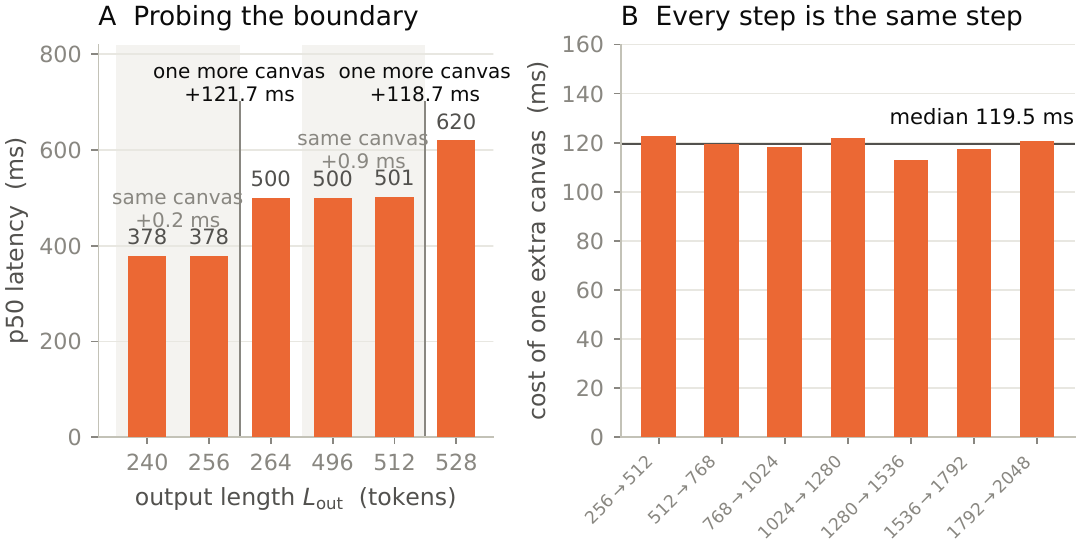
\includegraphics[width=\linewidth]{figures/fig2_canvas_edges.png}
\caption{The staircase probed at canvas boundaries. \textbf{A:}
latency is flat inside a canvas and jumps at the boundary --- tokens
within a canvas are free. \textbf{B:} all seven canvas transitions
out to $L{=}2048$ fall within an $8\%$ spread (median \dgStep\,ms),
so one canvas costs about the same wherever it sits. That regularity
is why the second term of Eq.~\ref{eq:dg} is a single constant
($K{=}8$, BGL, $n{=}200$).}
\label{fig:edges}
\end{figure}

\subsection{What the base is made of}

Fitting $T_{\textsc{dg}}(K) = \alpha + \beta K$ to measurements at
$K{=}2$ and $K{=}8$ splits the base into a $K$-independent floor of
$\approx$143\,ms ($38\%$) and per-step work of $\approx$236\,ms
($62\%$); see Appendix~\ref{app:decomp}. The per-step share is the
larger one because each denoising step re-attends the whole prompt,
prefill is paid $K$ times, not once. So if the prompt KV were cached
across denoising steps, most of that $62\%$ would collapse and the
base could fall toward the $\sim$150\,ms floor, taking $L^{*}$ down
with it. We treat the measured base as the operative number.

\paragraph{Generalisation.}

Both laws generalise from BGL to HDFS within 2\%: the DG canvas step
is \bglStep\,ms on BGL against \hdfsStep\,ms on HDFS, a $1.7\%$
difference at matched $K{=}8$ and canvas size. The step is a model
property, not a data property, which is why it barely moves. Two
caveats bound this: HDFS is the 2{,}000-line LOGHUB
sample~\cite{loghub} over a full corpus, evaluated at
$n{=}100$--$200$ per cell against BGL's $n{=}200$; the AR-30B was
re-measured on HDFS (p50 1082\,ms, CI [1078, 1106]) but the AR
generalisation slope was fitted on the dense AR-3B. So the
\emph{shape} transfers across corpora on both arms, and the AR-30B
point estimate confirms it, but the AR slope constant is from the
smaller model.

The shape also transfers across \emph{tasks}: on HumanEval code
generation (Appendix~\ref{app:humaneval}), AR-30B decodes at
6.4\,ms/token (vs 7.2 on logs) and DG is a flat 280\,ms staircase. The
AR/DG ratio is 2.9$\times$ (vs 2.5$\times$ on logs), in the same range.
Code is the ideal second task because truncation is catastrophic
(\texttt{SyntaxError}), making the completeness guarantee concretely
visible.

